\documentclass{report}
\usepackage[margin=1in, paperwidth=8.5in, paperheight=11in]{geometry}
%Math packages%
\usepackage{amsmath}
\usepackage{amsthm}
\usepackage{amssymb}
%Spacing%
\usepackage{setspace}
%Package to adjust indentation%
\usepackage{changepage}
\onehalfspacing
%Lecture number%
\newcommand{\lectureNum}{13}
%Variables - Date and Course%
\newcommand{\curDate}{February 14, 16, 2017}
\newcommand{\course}{CS 240}
%Defining the example tag%
%\theoremstyle{definition}%
\newtheorem{ex}{Example}[section]
%Setting counter given the lecture number%
\setcounter{chapter}{\lectureNum{}}
%Package to insert code%
\usepackage{listings}
\usepackage{courier}
\usepackage{xcolor}
\lstset { 
    tabsize=2,
    breaklines=true,
    language=C++,
    backgroundcolor=\color{blue!8}, % set backgroundcolor
    basicstyle=\footnotesize\ttfamily,% basic font setting
}
%Package to draw trees%
\usepackage{tikz}


\begin{document}
%Note title%
\begin{center}
\begin{Large}
\textsc{\course{} | Lecture 13 \& 14}
\end{Large}
\end{center} 
\noindent \textit{Bartosz Antczak} \hfill
\textit{Instructor: Eric Schost} \hfill
\textit{\curDate{}}
\rule{\textwidth}{0.4pt}

% Actual Notes%
\section{Hashing}
\textbf{Hashing} is another implementation of a dictionary.
\subsubsection{Structure}
We first outline a requirement: for any given $M \in \mathbb{N}$ (i.e., any piece of data), there exists a key as an integer with $0 \leq k < M$. This data structure is an array of values $A$ with size $M$. We first consider the hash function:
$$h: U \rightarrow \{0, 1, \cdots, M-1\}$$
Where $U$ is some universe. Generally $h$ is not injective, so many keys can map to the same integer.\\
Its structure is very simple: it is an array $T$ of size $M$, and any item with key $k$ is stored in $T[h(k)]$. In theory, all of its methods (insert, search, and delete) should cost $O(1)$.\\
Immediately, however, we spot an issue: how do we deal with collisions? (i.e., when $h(k_1) = h(k_2)$). There are two solutions: \textit{buckets} and \textit{open addressing}:
\subsection{Buckets (or Chaining)}
This method involves every table entry being what's called a ``bucket" containing zero or more key-value pairs. The simplest approach is to structure each bucket using an unordered linked list.
\begin{ex}
A hash table using buckets
\end{ex}
\begin{center}
\begin{figure}[ht]
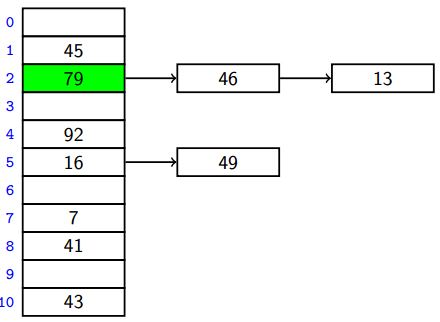
\includegraphics[scale=0.5]{table1.jpg}
\end{figure}
\end{center}
\subsubsection{Analysis}
\begin{itemize}
\item \texttt{search}: $\Theta(1 + \alpha)$ average case, $\Theta(n)$ worst-case
\item \texttt{insert}: $O(1)$ worst-case, since we always insert in front
\item \texttt{delete}: same cost as search
\end{itemize}
\subsection{Open Addressing}
The main idea is that each hash table enty holds only one item but any key $k$ can go in multiple locations. To search for and insert an element into the table, we follow a \textit{probe sequence} of possible locations for key $k$. The simplest idea is what's called linear probing. \textit{An example can be seen on the course slides.}
\subsection{Double Hashing}
Say we have two hash functions that are independent. The probability that $h_1(k) = a$ and $h_2(k) = b$ for any particular $a$ and $b$ is:
$$\frac{1}{M^2}$$
For double hashing, we define $h(k,i) = h_1(k) + i \cdot h_2(k) \mod M$. The basic methods (search, insert, and delete) work just like for linear probing.
\subsection{Cuckoo Hashing}
This is a relatively new idea, discovered in 2001. Again, we use two independent hash functions $h_1$ and $h_2$.
%END%
\end{document}